\documentclass[11pt, reqno]{article}    % use "amsart" instead of "article" for AMSLaTeX format
\usepackage{my_packages}
\usepackage{tikz_packages}
\usepackage[american,siunitx]{circuitikz}
\usepackage{pgfplots}
\pgfplotsset{compat=1.14}
\usepackage[explicit]{titlesec}


\title{MAE 3145: PREDICT}
\author{Shankar Kulumani}
\date{Fall 2017}                          % Activate to display a given date or no date

\begin{document}
\begin{center}
{\Large \textbf{MAE3145: PREDICT}}
\end{center}
\subsection*{Description}
You are tasked to support teh elite Space Surveillance Reconstitution Team (SSRT) as an orbital analyst.
The SSRT will deploy to setup a remote space tracking capability when threat levels against the US indicate an attack in imminent.
As a SSRT member, it is your responsibility to develop software to locate satellite fom an Earth location.
In particular, SSRT's tacitcal terminal requires topocentric range, azimuth, and elevation to point its new secret tracking instruent.
Your program must compute and output this information at \underline{two minute intervals} each time the tactical \underline{terminal is in darkness} and the \underline{satellite is above the terminal's local horizon at a reasonable range}.
In addition, your program must determine if the statellite is visible to the tactical terminal, i.e. terminal in the dark, satellite illuminated by the sun, elevation angle greater than or equal to \SI{10}{\degree}, range less than \SI{1500}{\kilo\meter}.
If the satellite is in sunlight, SSRT members can operate teh terminal's new pointing instrument in one of three classified modes.

The SSRT's existence must be kept secret.
Thus, to validate your software \textbf{you must} view a low Earth orbiting satellite based on your program results.
In addition, if you know someone located at least \SI{100}{\kilo\meter} from our training site, and this person can be sworn to secrecy, give them your program results so they too can view a satellite.
Another person viewing a satellite based on yoru results will serve as a independent validation of your work.

As with all practical programming applications, there are three steps to this project:
\begin{enumerate}
    \item You will develop the correct algorithm and accomplish som hand calculations to provide a bsis to test your coded subroutines,
    \item You will code all subroutines, checking their output with that of your hand calculations to validate each subroutine as you go, eventually putting together the complete program and matching a provided single satellite data file perfectly,
    \item You will slightly alther this working program to accept a data file of hundres of real satellits, identify a viable vehicle to personally view, and go view it.
\end{enumerate}

The data required to run your program is located on \href{https://github.com/fdcl-gwu/MAE3145_library}{MAE3145: Astro Library}.
I will update these files throughout the semester.
The data comes from JSPOC's Two-Line Element Sets (TLEs), which are typically found in terms of three lines of data.
Each data set contains the 100+ brightest active payloads that JSPOC tracks.
However, not all satellites will be visible to the naked eye.

The TLE files are given in a very specifc format as shown in~\cref{fig:tle}. 
The following describes each paramerter contained in the TLEs.
Some of these numbers will not be used in your program. 
You may also get teh latest TLEs yourself at \href{www.clestrak.com}{celestrak.com}.
There are many references for the TLE description available in textbooks or online, but one is available \href{https://goo.gl/W6MZb2}{https://goo.gl/W6MZb2}.

\begin{figure}
    \centering
    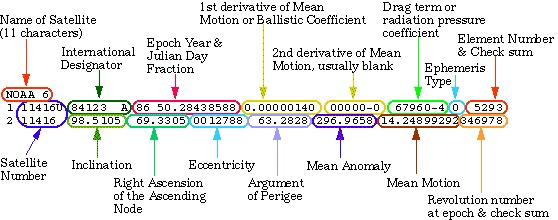
\includegraphics[width=\textwidth, keepaspectratio]{figures/tle.jpeg}
    \caption{TLE Format\label{fig:tle}}
\end{figure}
\subsection*{Project Requirements}
After completing the project you must submit the hard copies of your work:
\begin{itemize}
    \item Complete algorithms for the main driver script as well as a seperate algorithm for each sub-function that you develop.
        Someone totally unfamiliar with astrodynamics should be able to duplicate your program in any computer language.
    \item Clear, concise and properly documented and tested code
    \item Correct outputs from your program which matches the test cases
    \item Any additional test cases you may have used. 
        Explain why you did or did not use any additional test cases.
\end{itemize}

\subsection*{Authorized Resources}
You may consult with your instructor, the course notes or other reference material, and other students. 
However, you \textbf{MAY NOT} copy another student or any other individuals code. 
The program you develop must be your own work.

\subsection*{Algorithm}

Write a structured algorithm that shows your approach to writing a computer program to perform all of the tasks described above.
This should be a complete \textbf{sequential} list of the \textbf{equations and logic (including loop)} that you will use to write your program.
The details of subalgorithms are only required for procedures that are new for this project, not those provided to you.
Instead, just mention what procedure will be used and the inputs and outputs of the procedure, e.g. ``Calculate orbital elements given position and velocity vectors using \texttt{rv2coe}''.

When completed, anyone should be able to write your code \textbf{solely} using the algorithm in \textbf{any} computer language of their choice.
Thus, define all symbols before you use them, and do not write the equations and logic using any language specific terminology, i.e. Something like `` Find the length of the vector using \texttt{norm(x)} '' is unacceptable.

Your algorithm must be \textbf{typed}, which will serve you well when you document your final code. 
This is also a good opportunity to practice your technical writing skills in \LaTeX.

\subsection*{Final COMFIX Deliverables}

Your program must process the \texttt{COMFIX.DAT} data file and generate output that matches the orbital elements in \texttt{COMFIX.OUT} to at least four decimal places. 
The input file, \texttt{COMFIX.DAT}, contains five observations, but your program should be able to process an arbitrary number of observations.

Submit the following on the due date:
\begin{itemize}
    \item Fully documented driver script
    \item Each procedure which you wrote or modified, fully documented (no library routines)
    \item Computer generated results which match \texttt{COMFIX.OUT}
\end{itemize}

\end{document}  
